%Quick Latex Template.
%Homeworks and reports. UTP-2016
%feedback:hfjimenez@utp.edu.co
\documentclass{article}									%Document class.
\usepackage[utf8]{inputenc}								%Tildes.
\usepackage{gensymb}		
\usepackage{graphicx}									%Images in the paper.
\usepackage{authblk}						
\usepackage{float}										% Image will be in the same place as you want.!!! x-/
\usepackage[table,xcdraw]{xcolor}

\title{Laboratorio 11. Radioactividad}
\author{Carlos Alberto Dagua Conda, Héctor Fabio Jiménez Saldarriaga, \\Juan Camilo Castrillon,\thanks{carlosdaguaco@utp.edu.co, hfjimenez@utp.edu.co, jucacastrillon@utp.edu.co} }

\date{Abril 2016}
\begin{document}
\maketitle

\section{Abstract}
In this paper we study experimentally the phenomena of Radioactivity, meaning that it refers to the particles which are emitted from nuclei as a result of nuclear instability.The different types of radioactivity lead to different decay paths which transmute the nuclei into other chemical elements. Examining the amounts of the decay products makes possible radioactive dating.Radiation from nuclear sources is distributed equally in all directions, obeying the inverse square law. We probe this using the Geiger–Müller tube that it's used for the detection of $\gamma$(\textit{gamma}) radiation, $X$-rays, and $\alpha$(\textit{alpha}) and $\beta$(\textit{beta}) particles, analyse and conclude.
\section{Introducción}
La radiactividad o radio actividad es un proceso físico natural y espontáneo, por el cual algunos elementos, llamados radiactivos, emiten radiaciones.El fenómeno de la radiación consiste en la propagación de energía en forma de ondas electromagnéticas o partículas subatómicas a través del vacío o de un medio material.
Teniendo presente que el decaimiento beta es un proceso mediante el cual un nucleido o núclido inestable emite una partícula $\beta$ (un electrón o positrón) para compensar la relación de neutrones y protones del núcleo atómico. \textbf{Henri Becquerel}, mientras experimentaba con fluorescencia, descubrió accidentalmente que el uranio impresionaba una placa fotográfica, envuelta con papel negro, con una radiación desconocida que no pudo ser considerada como rayos X. \newline
Tiempo después \textbf{Ernest Rutherford} continuó estos experimentos y descubrió dos tipos diferentes de radiación:
\begin{enumerate}
\item partículas alfa que no aparecen en las placas de Becquerel porque eran fácilmente absorbidas por las envolventes negro;
\item partículas beta que son 100 veces más penetrantes que las partículas alfa.
\end{enumerate}
\begin{figure}[H]
  \centering
     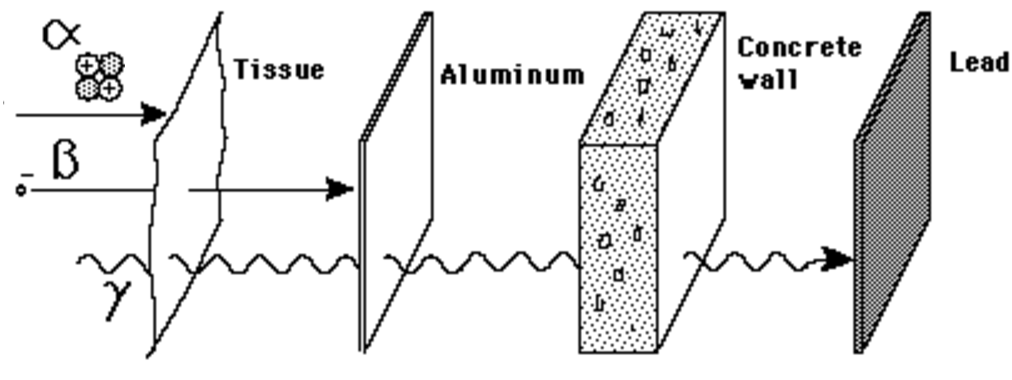
\includegraphics[width=0.97\textwidth]{radpen}
  \caption{Penetración de materiales, partículas Alfa, Gamma, Beta. Gamma es la mas penetrante.}
      \label{fig:penetracion}
\end{figure}
\begin{figure}[H]
  \centering
     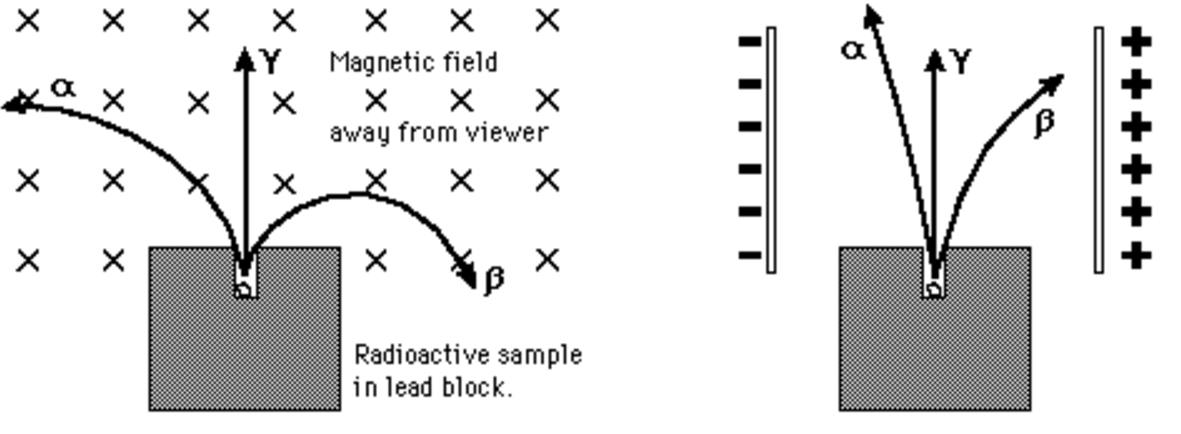
\includegraphics[width=0.97\textwidth]{alpbet}
  \caption{Alfa, Beta, y Gamma.}
      \label{fig:particulas}
\end{figure}

En esta practica de laboratorio experimentalmente utilizamos la muestra \textbf{\textit{TI-204}} utilizando el tubo GEIGER que exhibe un efecto \textit{plateau}, se utilizan diferentes bloqueadores, se mide la energía de decaimiento $\beta$, absorción de radiación y   comprobamos la ley del cuadrado inverso con la distancia, con su gráfica correspondiente.
 $$\\$$
 \subsection{Objetivos Practica}
 \begin{itemize}
	\item Determinar el valor de la radiación de fondo en el laboratorio
	\item Determinar si la ley del cuadrado inverso se aplica a la radiación emitida por sustancias radioactivas.
	\item Hallar la energía de decaimiento beta para la muestra TI-204
	\item Estudiar las características de absorción de los rayos $\beta$, $\alpha$ y $\gamma$.
\end{itemize}
 \subsection{Materiales Utilizados para la Práctica}
\begin{itemize}
\item Contador de Radiación Leybold Didactic 575471 NA
\item Tubo contador GEIGER Leybold Didactic 55901 (voltaje máximo 500 V)
\item Portamuestras
\item Muestras Radioactivas de Cs-137, Tl-204, Sr-90
\item Caja con absorbedores
\end{itemize}
%$\\$
%$\\$
\section{11.7 Análisis}
\subsection{11.7.1}
La radiación de fondo esta constituida por cierta variedad de radiación natural existente en el ambiente la cual es captada por el sensor causando errores en la medida de la radiación de muestras de baja actividad.\\Para Calcular el valor promedio de la radiación experimentalmente del laboratorio realizado  se obtuvieron valores \textbf{4} muestras, presentada en la tabla \ref{my-label} :

\begin{table}[H]
\centering
\begin{tabular}{|c|c|}
\hline
Tiempo            & Radiación de Fondo (Counts) \\ \hline
100s              & 27                         \\ \hline
100s              & 14                         \\ \hline
100s              & 18                         \\ \hline
100s              & 32                         \\ \hline
\textbf{Promedio}CPM & 22,75                      \\ \hline
\end{tabular}
\caption{Recolección de datos experimentales, Radiación de Fondo.}
\label{my-label}
\end{table}
Teniendo en cuenta que el promedio es $$Promedio = 22,75$$
sera el valor que seguiremos usando para realizar nuestros cálculos.
$$$$
$$$$
\subsection{11.7.2}
Se presenta la siguiente tabla obtenida, presenta la medida de radioactividad y :
\begin{table}[H]
\centering
\begin{tabular}{|l|l|l|l|l|l|}
\hline
\multicolumn{6}{|c|}{\textbf{Ley del Cuadrado Muestra TI-204}}  \\ \hline
\multicolumn{1}{|c|}{\textbf{Ranura}} & \multicolumn{1}{c|}{\textbf{Distancia D}} & \multicolumn{1}{c|}{\textbf{1/D\textasciicircum 2}} & \multicolumn{1}{c|}{\textbf{CPM}} & \multicolumn{1}{c|}{\textbf{\begin{tabular}[c]{@{}c@{}}CPM- Radiacion\\   de Fondo\end{tabular}}} & \multicolumn{1}{c|}{\textbf{\begin{tabular}[c]{@{}c@{}}Incertidumbre\\   CPM\end{tabular}}} \\ \hline
10   & 10,5             & 0,009           & 268         & 245      & 15,65              \\ \hline
9    & 9,5              & 0,011           & 306         & 283      & 16,82              \\ \hline
8    & 8,5              & 0,013           & 389         & 366      & 19,13              \\ \hline
7    & 7,5              & 0,017           & 495         & 472      & 21,72              \\ \hline
6    & 6,5              & 0,023           & 674         & 651      & 25,51              \\ \hline
5   & 5,5               & 0,033           & 986         & 963      & 31,03              \\ \hline
4   & 4,5               & 0,049           & 1500        & 1477     & 38,43              \\ \hline
3   & 3,5               & 0,081           & 2496        & 2473     & 49,72              \\ \hline
2   & 2,5               & 0,16            & 4891        & 4868     & 69,77              \\ \hline
1   & 1,5               & 0,44            & 13433       & 13410    & 115,8              \\ \hline
\end{tabular}
\caption{Ley del Cuadrado inverso, Muestra TI-204}
\label{my-label}
\end{table}
\subsection{11.7.3}
La gráfica de la ley del inverso del cuadrado, y sus actividades observadas en CPM del inverso de la distancia al cuadrado de la muestra al tubo GEIGER.
\begin{figure}[H]
  \centering
     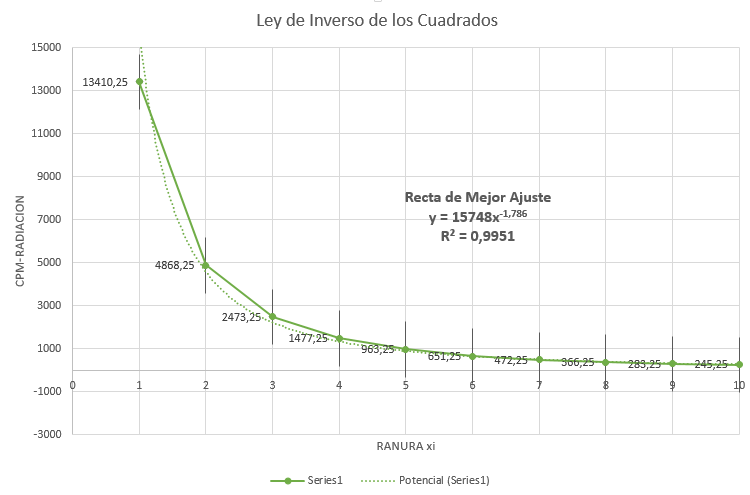
\includegraphics[width=0.97\textwidth]{cuadradosinverso}
  \caption{Representación Gráfica del inverso de los cuadrados.}
      \label{fig:cuadrado}
\end{figure}
$$\\$$
\begin{figure}[H]
  \centering
     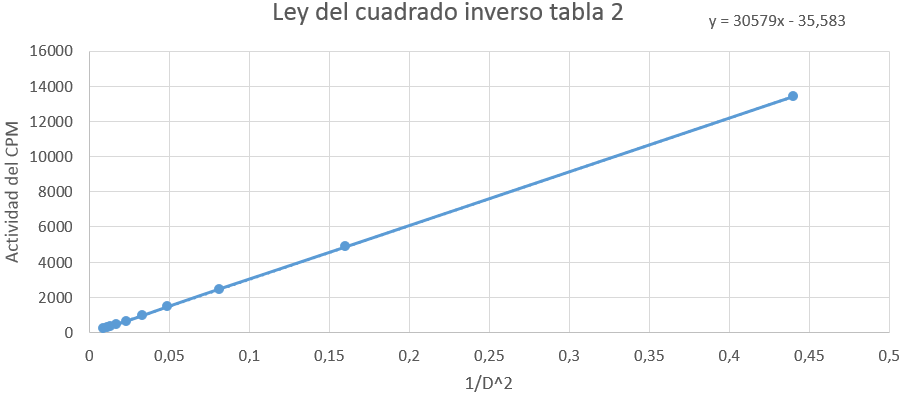
\includegraphics[width=0.97\textwidth]{gra2inverso}
  \caption{Representación Gráfica del inverso de los cuadrados.}
      \label{fig:cuadrado}
\end{figure}

\subsection{11.7.4}
Los datos siguientes corresponden a la absorción de radiación $\beta$ en función a la densidad de diferentes bloqueadores ubicados en la ranura 2, y la muestra  \textbf{ti-204} ubicada en la ranura 3.
\begin{table}[H]
\centering
\begin{tabular}{|c|l|l|l|l|}
\hline
\multicolumn{5}{|c|}{Absorción de Radiación RANURA 3}    \\ \hline
\textbf{Placa}     & \multicolumn{1}{c|}{\textbf{CPM}} & \multicolumn{1}{c|}{\textbf{\begin{tabular}[c]{@{}c@{}}CPM - Radiacion\\   de Fondo\end{tabular}}} & \multicolumn{1}{c|}{\textbf{\begin{tabular}[c]{@{}c@{}}Incertidumbre\\   CPM\end{tabular}}} & \multicolumn{1}{c|}{\textbf{logaritmo}} \\ \hline
\textbf{Sin placa} & 2380                              & 2358                                                                                               & 48,55                                                                                       & 3,37                                    \\ \hline
\textbf{A}         & 2134                              & 2112                                                                                               & 45,95                                                                                       & 3,32                                    \\ \hline
\textbf{B}         & 2139                              & 2117                                                                                               & 46,01                                                                                       & 3,33                                    \\ \hline
\textbf{C}         & 1922                              & 1900                                                                                               & 43,58                                                                                       & 3,28                                    \\ \hline
\textbf{D}         & 1566                              & 1544                                                                                               & 39,29                                                                                       & 3,19                                    \\ \hline
\textbf{E}         & 494                               & 472                                                                                                & 21,72                                                                                       & 2,67                                    \\ \hline
\textbf{F}         & 233                               & 211                                                                                                & 14,52                                                                                       & 2,32                                    \\ \hline
\textbf{G}         & 94                                & 72                                                                                                 & 8,48                                                                                        & 1,86                                    \\ \hline
\textbf{H}         & 45                                & 23                                                                                                 & 4,79                                                                                        & 1,36                                    \\ \hline
\textbf{I}         & 29                                & 7                                                                                                  & 2,64                                                                                        & 0,85                                    \\ \hline
\textbf{J}         & 27                                & 5                                                                                                  & 2,23                                                                                        & 0,70                                    \\ \hline
\textbf{S}         & 24                                & 2                                                                                                  & 1,41                                                                                        & 0,30                                    \\ \hline
\textbf{T}         & 23                                & 1                                                                                                  & 1                                                                                           & 0,00                                    \\ \hline
\end{tabular}
\caption{Uso de diferentes bloqueadores en conjunto con la muestra TI-204.}
\label{bloqueador}
\end{table}
$$$$
A continuación se presenta la relación de densidad para cada bloqueador correspondiente:
\begin{table}[H]
\centering
\begin{tabular}{|c|c|}
\hline
\multicolumn{2}{|c|}{\textbf{Materiales}} \\ \hline
Placa                & Densidad           \\ \hline
\textbf{A}           & 4,5                \\ \hline
\textbf{B}           & 6,5                \\ \hline
\textbf{C}           & 14,1               \\ \hline
D                    & 28,1               \\ \hline
\textbf{E}           & 59,1               \\ \hline
\textbf{F}           & 102                \\ \hline
\textbf{G}           & 129                \\ \hline
\textbf{H}           & 161                \\ \hline
\textbf{I}           & 206                \\ \hline
\textbf{J}           & 258                \\ \hline
\textbf{S}           & 3632               \\ \hline
\textbf{T}           & 7435               \\ \hline
\end{tabular}
\caption{Características de los Bloqueadores utilizados en la practica experimental de laboratorio.}
\label{my-label}
\end{table}
\textbf{Absorción de radiación Beta}\\
Con la ecuación de esta recta, se deduce el valor de la densidad del bloqueador en el punto de intersección con x (llamado D) y se reemplazó en la siguiente relación empírica para la energía de decaimiento $\beta$:
\begin{equation}
Em=1,84D+0,212
\label{eq1}
\end{equation}
Se tiene la ecuación 
$$f(x)=-0,0125x+3,4537$$
Haciendo la igualdad cero se tiene que $$0=-0,0125x + 3,4537$$Luego despejando $x$
$$\textbf{x}=\frac{3,4537}{0,0125}$$ se obtiene$$\textbf{x}=276.296$$Reemplazando en la ecuación \ref{eq1} :
\begin{equation}
Em=1,84(0,276296)+0,212
\label{eq2}
\end{equation}
\begin{equation}
  \textbf{Em}=0,7093328  \ MeV 
\label{eq3}
\end{equation}
\begin{figure}[H]
  \centering
     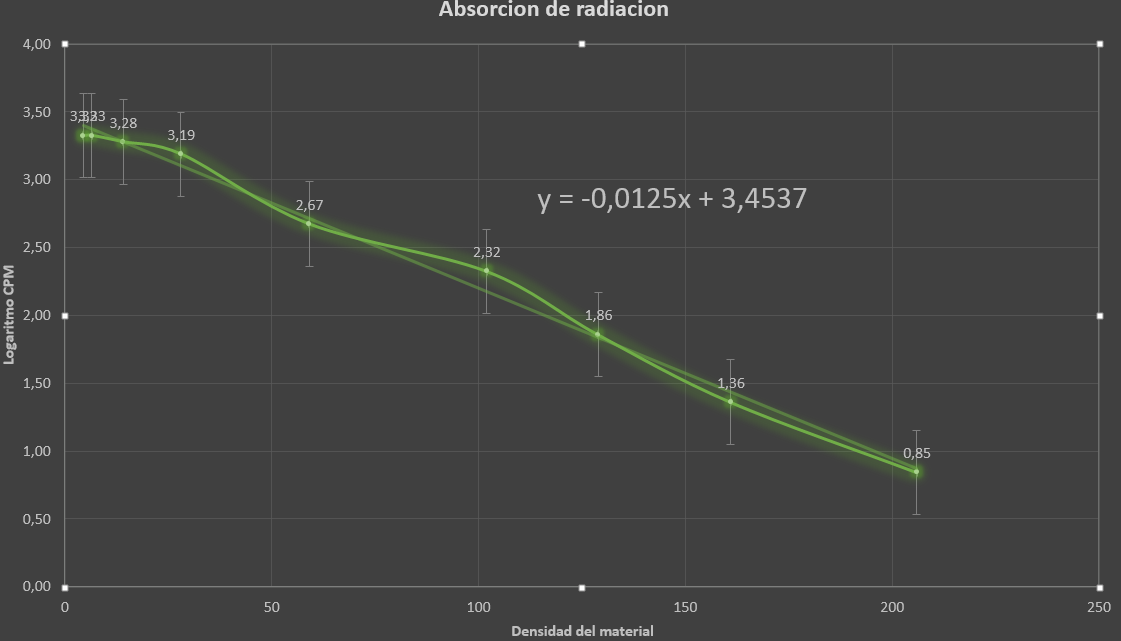
\includegraphics[width=0.97\textwidth]{absorcion}
  \caption{Representación Gráfica del logaritmo de la actividad en el eje y en función de la densidad del bloqueador en el eje x. Mejor recta posible}
      \label{fig:absorcion}
\end{figure}

\subsection{11.7.5}
Comparando el valor de $Em$ con su valor teórico. ($Emt = 0, 71$ MeV)

\begin{equation}
    \% Error = \frac{|Valor \ esperado-Valor \ experimental|}{Valor esperado}*100\%
\end{equation}
reemplazando en la ecuación anterior tenemos: 
\begin{equation}
    \% Error \% = \frac{|0,71-0,7093328|}{0,71}*100\% = \ 9,39\%
\end{equation}

\subsection{11.7.6}
La utilidad de conocer $Em$ (energía de decaimiento beta) en el experimento de radioactividad  se debe a que con esta podemos saber cuánta desintegración tuvo el elemento; la energía de decaimiento beta se produce a causa de la interacción nuclear débil, existe decaimiento $\beta$- que es el modo más frecuente  la cual implica la emisión de un electrón negativo, un negatrón o partícula $\beta$ como consecuencia de la transformación en el núcleo de un neutrón en un protón, o viceversa ($\beta+^{1}$)  Este tipo de transformación nuclear implica la emisión de un positrón o partícula$\beta+$ como consecuencia de la transformación dentro del núcleo de un protón en un neutrón El resultado del decaimiento beta es un núcleo en que el exceso de neutrones o protones se ha corregido en dos unidades y por tanto resulta más estable.\\
\section{Conclusiones}
\begin{enumerate}
\item Se comprobó que existen ciertas clases de materiales los cuales impiden el paso de radiación y cuya eficiencia dependen también del grosor de dicho material
\item Se da a entender que cada ambiente o espacio de trabajo común desprende una radiación de fondo que aunque esta sea de pequeña escala, debe ser tenida en cuenta
\item Se comprobó la Ley del cuadrado inverso con la distancia, (la intensidad de la luz emitida por una fuente puntual disminuye con el cuadrado inverso de la distancia a la fuente).
\end{enumerate}
\section{Bibliografia}
$[1]$ Raymond A. Serway Physics for Scientists and Engineers with Modern Physics. 
$\\$
$[2]$ Ley General del Inverso del Cuadrado, hyperphysics.phy-astr.gsu.edu/hbasees/forces/isq.html
$\\$
$[3]$ Guía de laboratorio de física III, Universidad Tecnológica de Pereira.

\end{document}

